\documentclass[10pt,twoside,draft]{book}
\usepackage{../../thesis}

\makeindex
\begin{document}

\chapter{Preliminaries}
\label{chap:prelim}
The purpose of this short chapter is to introduce notions of dynamical systems that will be used throughout the exposition.
%Since each definition of chaos uses different ideas, rather than to introduce them here all at once, we introduce those ideas as required on the fly.
%The reader may prefer to come back to this chapter as he/she encounters unfamiliar notations.

\section{Topological Dynamical Systems}
\begin{definition}
  (Dynamical System)
  Let $X$ be a topological space, and $F: X \to X$ be a continuous mapping.
  A (topological) dynamical system is defined to be $(X, F)$.
  %\index{}
\end{definition}
\begin{remark}
  We will often use a metric space as our topological space.
\end{remark}
%
\begin{definition}
  (Iteration)
  Let $F: X \to X$ be a mapping.
  \textit{The $n$th iteration of F}, denoted $\itr{F}{n}$, is defined as follows
  \begin{equation*}
    \itr{F}{n} \ceq \underbrace{F \circ F \circ \cdots \circ F}_{n} .
  \end{equation*}
  Note that, if $F$ is continuous, then $\itr{F}{n}$ is continuous for any $n \in \N$.
\end{definition}
\begin{remark}
  We will never use the superscript notation to denote the exponentiation of a value (as in $F(x) = 2x$, then $F^2(x) = 4x^2$).
\end{remark}
%%%
\begin{definition}
  (Orbit)
  Let $F: X \to X$. 
  The \textit{orbit} of $x_0$ is defined as the sequence
  \begin{equation*}
    O_F(x_0) \ceq \seq{\itr{F}{n}(x_0)}{\infty}{n = 0}.
  \end{equation*}
  $O_F(x_0)$ will simply be denoted as $O(x_0)$ when there is no ambiguity in the choice of $F$.
  \label{def:orbit}
  \index{orbit}
\end{definition}
%%%
It is convenient for our purpose to extend the notion of metric to a point and an orbit.
\begin{definition}
  (Distance between a point and an orbit)
  Let $X$ be a metric space, and $F: X \to X$ be a mapping.
  For each $x,y \in X$, the metric between $O(x)$ and $y$ is defined as follows
  \begin{equation*}
    \metric{O(x),y} \ceq \sup\limits_{x' \in O(x)} \metric{x',y}.
  \end{equation*}
\end{definition}
%%%
\begin{definition}
  (Periodic points)
  Let $F: X \to X$ be a mapping, and $p$ be a point in $X$.
  If $\itr{F}{n}(p) = p$ for some $n > 0$, and $\itr{F}{m}(p) \neq p$ for each $1 \leq m < n$, then $p$ is called a periodic point of period $n$, or simply a $n$-periodic point.
  \label{def:porbit}
  \index{periodic points}
\end{definition}
%%%

In topological dynamical systems, we are interested in properties that are preserved under continuous mappings.
All definitions of chaos that we discuss in this book are topological invariants.
%Since properties that we are specifically interested are global properties of a given space, we will require a conjugacy to be surjective. 
\begin{definition}
  (Conjugacy)
  Let $F: X \to X$ and $G: Y \to Y$ be continuous mappings.
  We say that $G$ is \textit{semi-conjugate} to $F$ (by $\phi$), if there exists a continuous and surjective mapping $\phi: X \to Y$ such that $\phi\circ F = G\circ\phi$ (Figure~\ref{fig:conj}).
  Moreover, if $\phi: X \to Y$ is a homeomorphism, we say that $G$ is \textit{conjugate} to $F$.
  \index{conjugacy}
\end{definition}
\begin{figure}[ht]
  \centering
  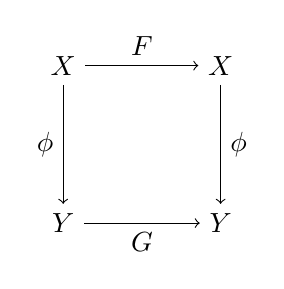
\begin{tikzpicture}[node distance=2cm, auto]
    \node (x1) {$X$};
    \node (x2) [right of=x1] {$X$};
    \node (y1) [below of=x1] {$Y$};
    \node (y2) [below of=x2] {$Y$};
    \draw[->] (x1) to node {$F$} (x2);
    \draw[->] (x1) to node[swap] {$\phi$} (y1);
    \draw[->] (y1) to node[swap] {$G$} (y2);
    \draw[->] (x2) to node {$\phi$} (y2);
  \end{tikzpicture}
  \caption{Conjugacy between $(F, X)$ and $(G, Y)$ via $\phi: X \to Y$.}
  \label{fig:conj}
\end{figure}
%%%
We often think of two dynamical systems being ``the same'' when there exists a (homeomorphic) conjugacy between them, since they possess the same topological properties.

\bibliographystyle{../../pjgsm}
\bibliography{../../bibliography/thesis}

\printindex
\end{document}

%\section{Metric Spaces}
%This section introduces notations used in the rest of the book.
%Also, we prove the contraction fixed point theorem.
%
%\begin{definition}
%  (Metric space)
%  A binary operation $\metric{}$ is called a \textit{metric} if it satisfies the following properties for each $x,y,z \in X$:
%  \begin{enumerate}
%    \item $\metric{x,y} = 0 \mbox{ iff } x = y$
%    \item $\metric{x,y} = \metric{y,x}$
%    \item $\metric{x,y} \leq \metric{x,z} + \metric{z,y}$.
%  \end{enumerate}
%  A \textit{metric space} $X$ is a set equipped with a metric.
%  %\index{metric}
%\end{definition}
%%%
%\begin{definition}
%  (Neighborhood)
%  Let $X$ be a metric space, and $\delta$ be a metric on $X$.
%  For $\epsilon \in \R$, and $x \in X$, a (open) \textit{neighborhood} $\oball{\epsilon}{x}$ is defined as 
%  \begin{equation*}
%    \oball{\epsilon}{x} \ceq \setst{y}{\metric{y,x} < \epsilon}
%  \end{equation*}
%  I shall use the terms ``open ball'' and ``neighborhood'' interchangeably.
%\end{definition}
%%%
%\begin{definition}
%  (Closed neighborhood)
%  Let $X$ be a metric space, and $\delta$ be a metric on $X$.
%  For $\epsilon \in \R$, and $x,y \in X$, a \textit{closed neighborhood} $\cball{\epsilon}{x}$ is defined as the closure of the corresponding open neighborhood, i.e.
%  \begin{equation*}
%    \cball{\epsilon}{x} \ceq \cl(\oball{\epsilon}{x}).
%  \end{equation*}
%\end{definition}

%\begin{definition}
%  (Diameter of an set)
%  We denote the \textit{diameter} of $A \subseteq X$ by $\diam(A)$, and is defined as
%  \begin{equation*}
%    \sup\limits_{x,y \in A} \metric{x,y}.
%  \end{equation*}
%
%\end{definition}

%\begin{definition}
%  (Lipschitz constant; Contraction)
%  Let $X, Y$ be metric spaces, and $\delta_X$ and $\delta_Y$ be corresponding metrics.
%  A map $F: X \to Y$ is said to be a \textit{Lipschitz map} or to satisfy the \textit{Lipschitz condition} iff there exists a $C \in \R$ such that for each $x_1, x_2 \in X$,
%  \begin{equation}
%    \delta_Y(F(x_1),F(x_2)) \leq C \delta_X(x_1, x_2). 
%    \label{eqn:lipcond}
%  \end{equation}
%  Clearly, a Lipschitz map is uniformly continuous.
%  We define the \textit{Lipschitz constant}, $\Lip(F)$, of $F$ as the greatest lower bound of the set of all $C$, i.e.
%  \begin{equation*}
%    \Lip(F) \ceq \inf\setst{C}{C \mbox{ satisfies } \eqref{eqn:lipcond}}.
%  \end{equation*}
%  Furthermore, $F$ is called a \textit{contraction} if $\Lip(F) < 1$.
%  \index{Lipschitz constant}
%\end{definition}
%%%

%\begin{theorem}
%  (Contraction Fixed Point Theorem)
%  Let $(X,\delta)$ be a complete metric space, and $K: X \to X$ a contraction with $\Lip(K) = C$.
%  Then, $K$ has a unique fixed point.
%  \label{thm:cfp}
%  \index{contraction fixed point theorem}
%  %
%  \begin{proof}
%    For any point $x_0 \in X$, define
%    \begin{equation*}
%      x_n \ceq \itr{K}{n}(x_0).
%    \end{equation*}
%    We have
%    \begin{equation*}
%      \delta(x_{n+1}, x_n) \leq C \delta(x_n, x_{n-1}),
%    \end{equation*}
%    which implies
%    \begin{equation*}
%      \delta(x_{n+1}, x_n) \leq C^n \delta(x_1, x_0).
%    \end{equation*}
%    For any $m > n$, we have
%    \begin{align*}
%      \delta(x_m, x_n) &\leq \sum\limits_n^{m-1} \delta(x_{i+1}, x_i) 
%        \leq (C^n + C^{n+1} + \cdots + C^{m-1}) \cdot \delta(x_1, x_0) \\
%        & = C^n (C^{0} + \cdots + C^{m-n-1} ) \cdot \delta(x_1, x_0) \\
%        & = \frac{C^n(1 - C^{m-n})}{1-C} \cdot \delta(x_1, x_0)
%        \leq \frac{C^n}{1-C} \cdot \delta(x_1, x_0).
%    \end{align*}
%    Therefore, $\set{x_n}$ is Cauchy.
%    Since $X$ is complete, the sequence converges to a point in $X$, say $x$.
%    Finally, 
%    \begin{equation*}
%      K(x) = \lim\limits_{n\to \infty} K(x_n) = \lim\limits_{n\to \infty} x_{n+1} = x.
%    \end{equation*}
%    Thus, $x$ is a fixed point for $F$.
%  \end{proof}
%\end{theorem}
%%%

